\documentclass[10pt, a4paper]{article}
\usepackage[utf8]{inputenc}
\usepackage[T1]{fontenc,url}
\usepackage{multicol}
\usepackage{multirow}
\usepackage{parskip}
\usepackage{lmodern}
\usepackage{microtype}
\usepackage{verbatim}
\usepackage{amsmath, amssymb}
\usepackage{tikz}
\usepackage{physics}
\usepackage{mathtools}
\usepackage{algorithm}
\usepackage{algpseudocode}
\usepackage{listings}
\usepackage{enumerate}
\usepackage{graphicx}
\usepackage{float}
\usepackage{hyperref}
\usepackage{tabularx}
\usepackage{siunitx}
\usepackage{fancyvrb}
%\usepackage{natbib}
%\bibliographystyle{dinat}
\usepackage[makeroom]{cancel}
\usepackage[margin=2.0cm]{geometry}
\usepackage{pdfpages}
\usepackage[margin=10pt, textfont={small, it}, labelfont={bf}, labelsep=endash]{caption}
\renewcommand{\baselinestretch}{1}
\renewcommand{\exp}{e^}
\renewcommand{\b}{\boldsymbol}
\newcommand{\h}{\hat}
\newcommand{\m}{\mathbb}
\newcommand{\half}{\frac{1}{2}}
\renewcommand{\exp}{e^}
\renewcommand{\bar}{\overline}
\setlength\parindent{0pt}


\begin{document}
\title{AST5220\\ Milestone III -- Pertubations}
\author{
    \begin{tabular}{r l}
        Jonas Gahr Sturtzel Lunde & (\texttt{jonassl})
    \end{tabular}}
% \date{}    % if commented out, the date is set to the current date

\maketitle
Code found at \url{https://github.com/asdfbat/AST5220/tree/master/Project}
\vspace{0.7cm}

\section{Introduction}
We have in previous milestones studied the cosmological evolution of the smooth universe, from the relative density functions and their effect on the curvature and conformal time in Milestone I, to the the free electron fraction and its resulting optical depth in Milestone II. In this milestone we introduce pertubations to our smooth universe, which is vital for the observed anisotropies in the cosmic microwave background radiation. This pertubation is naturally included in the Newtonian gauge, which leaves only two degrees of freedom in the line element, namely the two pertubation parameters $\Psi$ and $\Phi$.


\section{Theory}
\subsection{Gauge and metric}
In the newtonian Gauge, the metric takes the form of
\begin{equation}
    \begin{aligned}
        g_{00} &= - (1 + 2\Psi(\vec x,t)) \\ 
        g_{ij} &= \delta_{ij}a^2(1 + 2\Phi(\vec x, t))
    \end{aligned}
\end{equation}
with the off-diagonal elements being zero.

...




\section{Results}

\begin{figure}[H]
    \centering
    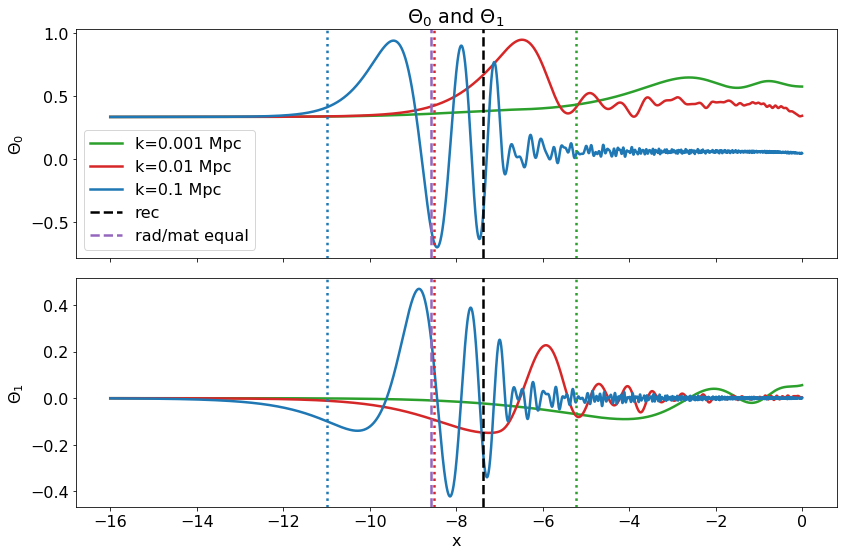
\includegraphics[scale=0.45]{../m3_figs/thetas.png}
    \caption{}
    \label{}
\end{figure}


\begin{figure}[H]
    \centering
    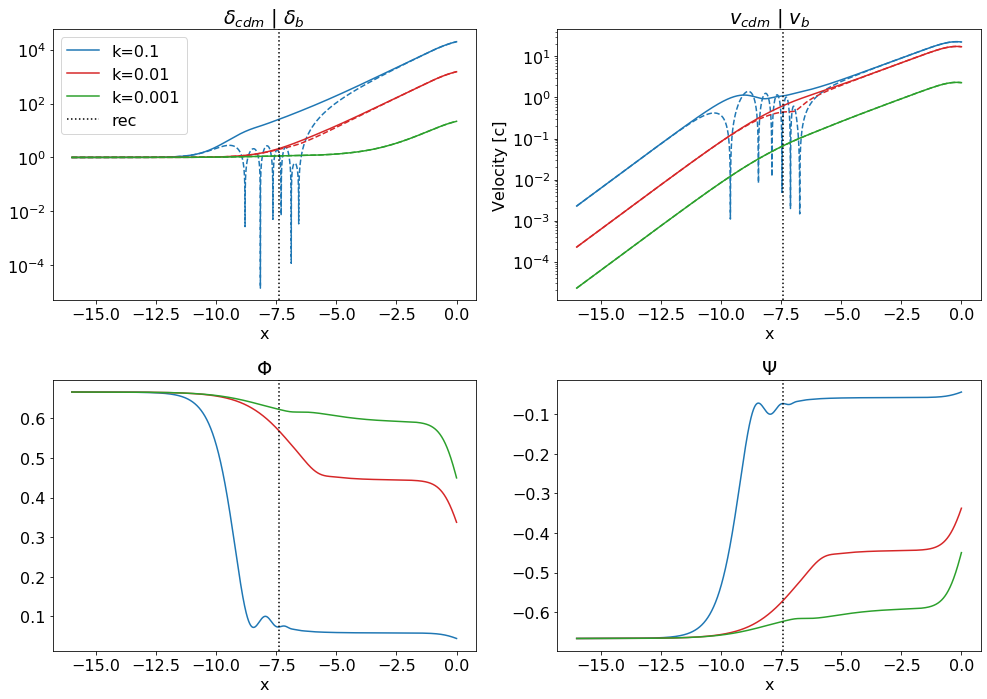
\includegraphics[scale=0.45]{../m3_figs/pertubations.png}
    \caption{}
    \label{}
\end{figure}


\bibliography{ref}
\bibliographystyle{plain}



\end{document}